\documentclass[]{bioinfo}
\usepackage[table,xcdraw]{xcolor}
\usepackage{caption}
\usepackage[subrefformat=parens]{subcaption}
\usepackage{hyperref}
\copyrightyear{2014}
\pubyear{2014}

\makeatletter
\let \@sverbatim \@verbatim
\def \@verbatim {\@sverbatim \verbatimplus}
{\catcode`'=13 \gdef \verbatimplus{\catcode`'=13 \chardef '=13 }} 
\makeatother

\begin{document}
\firstpage{1}

\title[3Dmol.js: Molecular Visualization with WebGL]{3Dmol.js: Molecular Visualization with WebGL}
\author[Rego and Koes]{Nicholas Rego\,$^{1,2}$ David Koes$^{1}$\footnote{to whom correspondence should be addressed}}
\address{$^{1}$Department of Computational and Systems Biology, University of Pittsburgh, Pittsburgh, PA 15260\\
$^{2}$Department of Biochemistry and Molecular Biophysics, University of Pennsylvania, Philadelphia, PA 19104}

\history{Received on XXXXX; revised on XXXXX; accepted on XXXXX}

\editor{Associate Editor: XXXXXXX}

\maketitle
\begin{abstract}
\section{Summary} 3Dmol.js is a modern, object-oriented JavaScript library that uses the latest web technologies
to provide interactive, hardware-accelerated three dimensional representations of molecular data without the
need to install browser plugins or Java.  3Dmol.js provides a full featured API for developers as well
as a straightforward declarative interface that lets users easily share and embed molecular data in websites.
\section{Availability} 3Dmol.js is distrubuted under the permissive BSD open source license.
Source code and documentation can be found at \url{http://3Dmol.csb.pitt.edu}
\section{Contact:} \href{dkoes@pitt.edu}{dkoes@pitt.edu}
\end{abstract}

\section{Introduction}
Molecular visualization is an essential tool for computational chemists and biologists. Due to the demanding nature of 3D graphics, most molecular viewers, such as PyMol\cite{delano2002pymol}, Chimera\cite{pettersen2004ucsf}, VMD\cite{humphrey1996vmd}, and Avogadro\cite{hanwell2012avogadro}, are desktop applications.  The need to install specialized applications and, in some cases, the restrictive nature of the software licenses, introduces hurdles to the sharing of molecular data.  Unlike a desktop application, a standards-based client-side web application comes pre-installed with every computer and mobile device with a modern web browser and can be seamlessly integrated into online environments for accessing and analyzing molecular data.


Currently, Jmol\cite{jmol,hanson2010jmol} is the most used web-based molecular viewer. Jmol is implemented as a Java applet and includes a custom rendering engine for efficiently rendering common molecular data representations such as spheres and sticks.  Due to this custom rendering engine and Java's optimizing just-in-time compiler, the performance of Jmol can approach that of native, desktop applications.  However, due to heavily publicized security failures, it can no longer be assumed that users have Java installed by default\cite{doomedjava}.  Even when Java is installed, users are presented with multiple security prompts that must be correctly dealt with before a Java applet, such as Jmol, can run.
To address these concerns, JSmol\cite{hanson2013jsmol} was developed. JSmol is largely the result of applying a Java to JavaScript translator to Jmol. As the \textit{de facto} web browser scripting language, JavaScript, unlike Java, is widely deployed and enabled by default.  However, particularly for large and complex visualizations, the performance of JSmol lags behind that of Jmol.

An alternative to the software-based rendering of Jmol/JSmol is to use hardware-accelerated graphics, as is done with desktop applications.  This is enabled by the recently adopted WebGL\cite{webgl} standard, which is now supported natively in the latest versions of all the major desktop and mobile browsers. GLmol\cite{glmol} is a WebGL based molecular viewer that uses the Three.js\cite{threejs} framework for interfacing with WebGL.  However, GLmol lacks a full featured API and the use of the Three.js library results in performance inefficiencies.



\section{3Dmol.js}

3Dmol.js is a pure JavaScript, hardware-accelerated, object-oriented molecular visualization library that enables web developers and casual users to visualize and interact with molecular data in any modern web browser with near native performance.  The focus of 3Dmol.js is providing a full-featured API for online high-performance molecular visualization. This allows 3Dmol.js to be integrated with other web applications that provide additional cheminformatics and analysis capabilities.
A variety of common styles are supported, as demonstrated by Figure~\ref{pic}.
3Dmol.js can be used to view molecular data by web application developers, HTML authors, and end users.  

\paragraph{JavaScript API}  JavaScript developers can use 3Dmol.js by including a single minified script and using the routines provided in the \texttt{\$3Dmol} namespace. There are routines to manipulate and style molecular data, generate molecular surfaces, create arbitrary shapes such as spheres and arrows, annotate the view with text and image labels, and install callback handlers for when a user interacts with the viewer contents (e.g., clicks on an atom).  An example of programmatically controlling a 3Dmol.js viewer to create the scene shown in Figure~\ref{pic} is provided in Figure~\ref{code}.

\paragraph{Embeddable Viewer} HTML authors do not need to use JavaScript to embed 3D viewers within their websites.  3Dmol.js will automatically turn any HTML element annotated with the \texttt{viewer\_3Dmoljs} class into a viewer.  The contents of the viewer are set and styled through the use of HTML \texttt{data} tags, as shown in Figure~\ref{embed}.  The molecular data can be retrieved from a remote URL or from an element that is embedded within the web page.

\paragraph{Hosted Viewer} End users may use 3Dmol.js through a hosted viewer as shown in Figure~\ref{url}. In this case, the molecular data is set and styled through a URL specification.  Data may be retrieved from a remote URL, such as a publicly accessible shared folder on cloud storage.  This allows users to easily share complex scenes without requiring that the recipients have any software other than a modern web browser. 




\begin{figure}
\centering
\begin{minipage}[b]{.9\linewidth}
\begin{subfigure}[b]{\linewidth} \centering
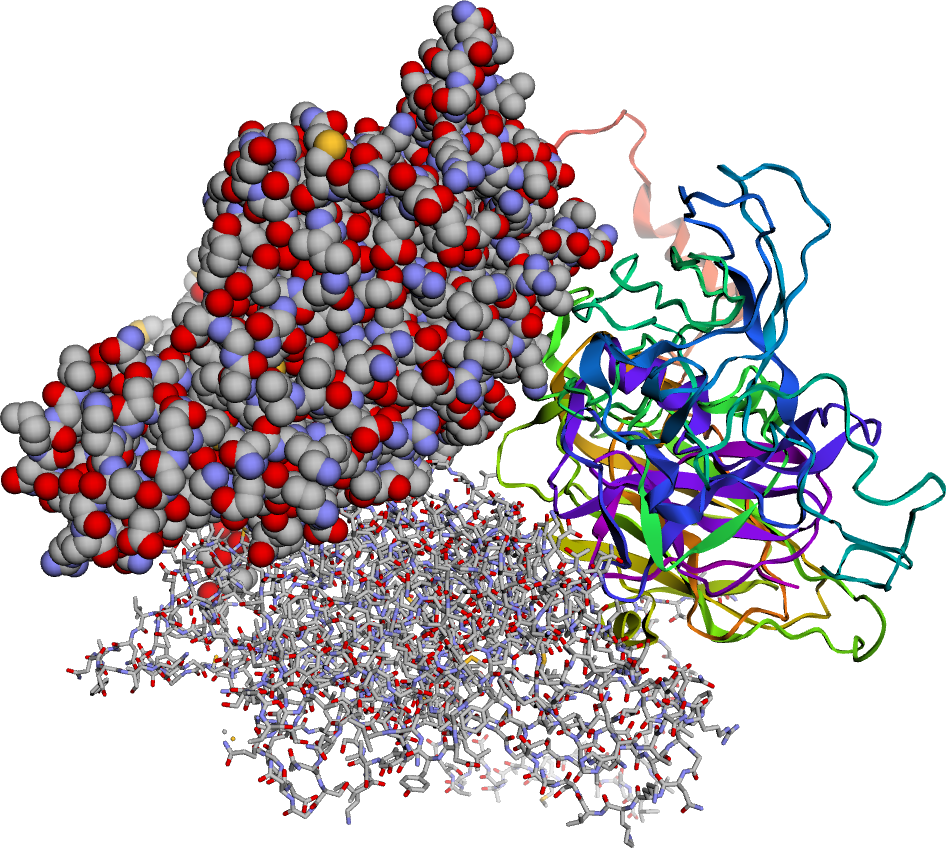
\includegraphics[width=\linewidth]{screenshot}
\caption{}\label{pic}
\end{subfigure}
\end{minipage}

\begin{minipage}[b]{\linewidth}

\begin{subfigure}[b]{\linewidth} \centering
\begin{verbatim}
$3Dmol.download('pdb:3M8L', viewer);
viewer.setStyle({chain:'A'}, {sphere:{} });
viewer.setStyle({chain:'B'}, 
            {cartoon:{color: 'spectrum'} });
viewer.setStyle({chain:'C'}, {stick:{} });
viewer.render();
\end{verbatim}
\caption{}\label{code}
\end{subfigure}

\begin{subfigure}[b]{\linewidth} \centering
\begin{verbatim}
<div style="height: 600px; width: 600px;" 
 class='viewer_3Dmoljs' data-pdb='3M8L'
 data-backgroundcolor='0xffffff'  
 data-select1='chain:A'
 data-style1='sphere'
 data-select2='chain:B'
 data-style2='cartoon:color=spectrum'
 data-select3='chain:C'
 data-style3='stick'></div>
\end{verbatim}
\caption{}\label{embed}
\end{subfigure}

\begin{subfigure}[b]{\linewidth} \centering
\begin{verbatim}
http://3dmol.csb.pitt.edu/viewer.html?
 pdb=3M8L&select=chain:A&style=sphere&
 select=chain:B&style=cartoon:color~spectrum&
 select=chain:C&style=stick
\end{verbatim}
\caption{}\label{url}
\end{subfigure}

\begin{subfigure}[b]{\linewidth} \centering
\begin{tabular}{ccccc}
 & \textbf{Jmol} & \textbf{JSmol} & \textbf{GLmol} &\textbf{3Dmol} \\
\textbf{Construct} & \textbf{0.136s} & 0.874s & 6.372s & 0.776s \\
\textbf{Rotate} & 0.053s & 0.207s & 0.673s & \textbf{0.002s} 
\end{tabular}
\caption{}\label{perf}
\end{subfigure}

\end{minipage}
\caption{\subref{pic} A capsid protein (PDB: 3M8L) with 12,375 atoms as rendered by 3Dmol.js.
This same scene can be generated \subref{code} programmatically in JavaScript, \subref{embed} from
within HTML, or \subref{url}  by specifying a properly formatted URL to the 3Dmol.js hosted viewer.
\subref{perf} The time required to create this scene and then rotate it for Jmol/JSmol 14.2.2, GLmol .47, and 
3Dmol.js.
}
\end{figure}




\section{Performance Comparison}

The performance of 3Dmol.js is compared to Jmol, JSmol, and GLmol in Figure~\ref{perf}.
The time to create the scene of Figure~\ref{pic}, which contains several visual styles applied to 12,375 atoms,
and then to perform a single rotation was measured using JavaScript wall clock time.  Firefox 31 on a 2.4Ghz Core Duo 2008 MacBook with 4GB of RAM running OS X 10.9.5
was used to time the operations and the average of the three best times of five trials is reported.

The initial creation time for a scene can be more time consuming in 3Dmol.js compared to a software-rendering approach like Jmol.
 The scene needs to be decomposed into a mesh of triangles since this is what is expected
by the graphics subsystem.  However, once a 3D scene is created, interactions with the scene that do not change its fundamental geometry,
such as rotating, translating, and zooming, are extremely fast since the 3D scene data is being managed by the native graphics subsystem.
This is demonstrated by the 2ms measured time for rotating the scene and is observed qualitatively by the smoothness with which a user 
 interacts with a 3Dmol.js viewer, even when the scene is quite complex. 

\section{Conclusion}
3Dmol.js is an high-performance interactive viewer for 3D molecular data that requires no plugins to work in modern desktop and mobile web browsers.
3Dmol.js provides a full-featured API to JavaScript developers, but can also be used by HTML authors and end users to share and distribute
3D visualizations of molecular data. 3Dmol.js is available under a permissive BSD open source license from \url{http://3dmol.csb.pitt.edu}.
 
\section*{Acknowledgements}

\paragraph{Funding\textcolon} 
This work was supported by the National Institute of Health [R01GM108340].
The content is solely the responsibility of the authors and does not necessarily
represent the official views of the National Institute of General Medical Sciences
or the National Institutes of Health.

\bibliographystyle{plain}
\bibliography{3dmol}
\end{document}